\documentclass[11pt]{article}
\usepackage[utf8]{inputenc}
\usepackage[T1]{fontenc}
\usepackage{mathptmx}
\usepackage{geometry}
\usepackage{mathtools}
\usepackage[english]{babel}
\usepackage{graphicx}
\usepackage[figurename=Gambar]{caption}
\usepackage{hyperref}
\usepackage{minted}
\usepackage{setspace}
\usepackage{color}
\usepackage[explicit]{titlesec}
\usepackage{tocloft}
\usepackage{titletoc}
\usepackage{indentfirst}
\usepackage{caption}
\usepackage{subcaption}
\usepackage{amsmath} 
\usepackage{pdfpages}
\usepackage{enumitem}


%\color{white}
%\pagecolor{black}

\hypersetup{colorlinks,
	citecolor=black,
	filecolor=black,
	linkcolor=black,
	urlcolor=black
}

\geometry{
	a5paper,
	left=30mm,
	right=25mm,
	top=15mm,
	bottom=15mm,
}

\date{}
%=============================================================================
% Modified Items

\providecommand{\keywordid}[1]{\textit{Kata Kunci: } #1}
\providecommand{\keyworden}[1]{\textit{Keywords: } #1}

\titleformat{\section}{}{}{0pt}{}
\titleformat{\subsubsection}{\small \bfseries}{\thesubsection}{0pt}{}

\renewcommand{\cftsecleader}{\cftdotfill{\cftdotsep}}
\renewcommand{\cftsubsecleader}{\cftdotfill{\cftdotsep}}

\makeatletter
\let\latexl@section\l@section
\def\l@section#1#2{\begingroup\let\numberline\@gobble\latexl@section{#1}{#2}\endgroup}
\makeatother

\addto\captionsenglish{\renewcommand{\contentsname}{}}
\addto\captionsenglish{\renewcommand{\listfigurename}{}}

\renewcommand{\cftsecfont}{\normalfont}
\renewcommand{\cftsecpagefont}{\normalfont}

\renewcommand{\thefigure}{\arabic{section}.\arabic{figure}}

\hyphenation{mening-katnya fuz-zy}


\numberwithin{equation}{subsection}

%=============================================================================
% Document Part

\begin{document}
	
	\onehalfspacing
	%=============================================================================
	% BAB I
	
	\newpage
	
	\pagenumbering{arabic}
	\setcounter{page}{9}
	
	\setcounter{section}{0}
	
	\setcounter{figure}{0}
	
	\section{Pendahuluan}
	
	\begin{center}
		{\large \textbf{BAB I}} \\
		{\large \textbf{Pendahuluan}}
	\end{center}
	
	\subsection{Latar Belakang}
	
	Kehidupan lansia di Indonesia meningkat seirinng meningkatnya jumlah kelahiran dan meningkatnya angka harapan hidup .
	hasil survey oleh  BPS  jumlah lansia mencapai 22.4 juta atau  8,69\%. pada tahun 2015\cite{Kesehatan}
	diperkirakan oleh oleh BPS pada tahun 2018 bisa mencapai 9,3\% dari penduduk seluruh indonesia atau 24.7 juta jiwa.
	Hal ini akan berakibat fatal apabila kehidupan lansia tidak dijaga dengan baik.
	Menjaga kesehatan lansia dalam usia yang sudah rentan baik di sebuah rumah atau gedung sangat perlu kehati-hatian.
	Contoh resiko jatuh lansia pada rumahan di Krasakan Lumbungrejo Tempel Sleman Yogyakarta dengan jumlah koresponden 100 orang, hasil yang di dapat  yaitu 16 orang (41\%) responden memiliki risiko jatuh sedang, 15 orang (38.5\%) memiliki risiko jatuh rendah
	dan yang terakhir 8 orang (20.5\%) memiliki risiko jatuh tinggi \cite{Utami2017a}
	Namun peningakatan resiko jatuh menjadi lebih besar jika lansia terdapat pada satu gedung atau rumah panti jompo.
	Contoh saja penelitian di panti social Tresna Werdha Budi Mulia 4 Margagguna, Jakarta Selatan dengan jumlah korespondsi 51 orang.
	Resiko jatuh dengan aktifitas fisik (73.7\%).
	Sehingga perhatian pada lansia harus sangat diperhatikan dan apabila lengah sedikit saja para lansia bisa saja terjatuh dan berakibat fatal.
	Dalam hal ini perhatian untuk di rumah di panti sosial menjadi kurang, ini bisa dilihat resiko jatuh pada lansia adalah (73.7\%).
	Sehubungan dengan pentingnya akan pendeteksi jatuh pada lansia maka alat yang tersedia terus berkembang mulai dari hardware sampai software yang digunakan.
	Contohnya saja pada tahun 2012 telah dibuat penelitian pendeteksi jatuh pada lansia menggunakan sistem fuzzy dan apabila terdeteksi dikomunikasikan melalui wireless xbee dan hasilnya sistem ini mempunyai akurasi minimal 86,6\%.
	Lalu pada tahun 2013 juga dibuat sistem pendeteksi jatuh dengan menggunakan fuzzy namun tidak mengirimkan data dan sekedar alarm di tubuh objek.
	Untuk akurasinya mencapai 92\%.
	Pada tahun 2014 untunk penelitian pendeteksi jatuh namun menggunakan type 2 fuzzy namun keakuratan justru hanya 80\%.
	Untuk tahun 2015 juga telah dibuat penelitian deteksi sistem jatuh menggunakan high level fuzzy petri net.
	Dan untuk sistem ini ke akurasiannya mencapai diatas 90\%.
	Untuk tahun 2016 dilakukan penelitian tentang teknik deteksi untuk jatuh menggunakan fuzzy model takagi sugeno dengan sensor accelerometer lalu pada tahun 2018 terdapat penelitian menggunakan metode non-intrusive deteksi jatuh pada lansia menggunakan logika fuzzy yang terdapat dua sensor untuk mendeteksi jatuh.
	Dua sensor ini yaitu sensor accelerometer dan sensor suara.
	Apabila terdeteksi maka akan dikirimkan melalui IoT ke perawat yang menjaga. Untuk sistem ini tingkta ke akurasian mencapai 80\%.

	Pada perkembangan alat pendeteksi jatuh dengan sensor accelerometer dan gyroscope  yang dibuat oleh Luthfi Fathurrahman sebelum memakai sistem adaptive neuro fuzzy inference system (ANFIS) hanya mempunyai sensitifitas  80\% dan spesitifitas 88\%.
	Ketika memakai sistem adaptive neuro fuzzy inference system (ANFIS) mempunyai kenaikan ketika nilai range of influence sebesar 0,1  maka sensitiitas menjadi 100% dan spesitifitas menjadi 91,67\%.
	Untuk range of influence sebesar 0,05  maka sensitifitas dan spesitifitas  menjadi 100.
	Dalam sistem sistem adaptive neuro fuzzy inference system (ANFIS) ini  mempunyai kekurangan yaitu belum bisa mendeteksi ketika objek terjatuh ke belakang sehingga nilai inilah yang harus di optimasi.
	Memaksimalkan keakurasi pendeteksian objek ketika terjatuh merupakan hal yang wajib yang harus dilakukan.
	Salah satu langkah dalam pendeteksian seperti menambah sensor.
	Sensor yang dimaksud adalah sensor suara, seperti pada jurnal yang dibuat oleh  Poi Voon Er dan Kok Kiong Tan kesalahan bisa ditekan sampai 20\% dan penambahan fitur optimasi untuk mengurangi kesalahan.
	Optimasi merupakan proses untuk memaksimalkan suatu perhitungan tertentu.
	Memaksimalkan suatu perhitungan tertentu maksudnya sistem fuzzy dalam penelitian sebelumnya tidak bisa mendeteksi jatuh kebelakang.
	Sehingga harapannya optimasi berjalan maksimal dan tidak ada kekurangan untuk logaritma fuzzy.
	Optimasi sendiri harus dilakukan dengan penuh percobaan dan perhitungan agar nilai hasil benar-benar merupakan nilai maksimal yang bisa dsilakukan.		
	
	\subsection{Rumusan Masalah}
	
		Adapun masalah dalam melakukan penelitian Tugas Akhir ini adalah sebagai berikut: :
	
	\begin{enumerate}[label=\alph*.]
		\item Bagaimanakah cara menentukan karakteristik kondisi orang saat terjatuh berdasarkan kegiatan yang sudah ditentukan?
		\item Bagaimana cara menentukan dan mengimplementasikan sebuah sistem pendeteksi kondisi terjatuh berbasis sensor posisi dam suara ?
		\item Bagaimana cara mengintegrasikan sensor posisi dan suara dengan fuzzy PSO (Particle Swarm Optimization) sebagai pengambil keputusan?
		\item Bagaimana cara menentukan performance dari sistem pendeteksi kondisi terjatuh berbasis accelerometer menggunakan fuzzy PSO (Particle Swarm Optimization)?
	
	\end{enumerate}
	
	
	
	\subsection{Tujuan Penelitian}
	
		Adapun masalah dalam melakukan penelitian Tugas Akhir ini adalah sebagai berikut: :
	
	\begin{enumerate}[label=\alph*.]
		\item Menentukan karakteristik kondisi orang saat terjatuh berdasarkan kegiatan yang sudah ditentukan
		\item Menentukan dan mengimplementasikan sebuah sistem pendeteksi kondisi terjatuh berbasis sensor posisi dan suara?
		\item Mengintegrasikan sensor posisi dan suara dengan fuzzy PSO (Particle Swarm Optimization) sebagai pengambil keputusan
		\item Menentukan performance dari sistem pendeteksi kondisi terjatuh berbasis accelerometer menggunakan fuzzy PSO (Particle Swarm Optimization)
		
	\end{enumerate}
	
	
	\subsection{Manfaat Penelitian}
	
Adapun batasan masalah yang digunakan dalam pengerjaan tugas akhir ini adalah sebagai berikut :
	
	\begin{enumerate}[label=\alph*.]
		
		\item Sensor yang digunakan adalah accelerometer, Gyroscope dan mic modul
		\item Metode yang digunakan dalam sistem pendeteksi terjatuh adalah PSO (Particle Swarm Optimization)
		\item Jenis kegiatan/ aktifitas objek untuk tujuan pengambilan data sudah ditentukan seperti berjalan, jogging, berdiri dan lain-lain
		\item Penempatan sensor untuk tujuan pengambilan data berada pada tiga posisi yaitu dada, reins dan paha
		
	\end{enumerate}

	\subsection{Sistematika Laporan}

Sistematika penulisan laporan tugas akhir adalah sebagai berikut:

\begin{enumerate}[label=\alph*.]
	
		
	\item Pada bab I yaitu pendahuluan yang terdiri dari latar belakang, rumusan masalah, tujuan, batasan masalah, dan sistematika laporan. 
	\item Pada bab II adalah teori penunjang dan dibahas mengenai teori-teori yang berkaitan dengan penelitian yang akan dilakukan, seperti teori accelerometer, mic, modul wifi, microcontroller dan android.
	\item Pada bab III yaitu metodologi penelitian yang berisi mengenai rancangan dari penelitian yang dilakukan, metode, dan langkah-langkah dalam penelitian. 
	\item Pada bab IV analisis data dan pembahasan yaitu berisi tentang analisis hasil perancangan sistem fuzzy PSO
	\item Pada bab V kesimpulan dan saran yang berisi kesimpulan tentang tugas akhir yang telah dilakukan berdasarkan data-data yang diperoleh serta diberikan saran sebagai penunjang maupun pengembangan untuk tugas akhir yang selanjutnya. 
	
	
\end{enumerate}
%=============================================================================

%\newpage
%\thispagestyle{plain}
%\mbox{}

%=============================================================================
% BAB II 

\newpage

\setcounter{figure}{0}

\section{TINJAUAN PUSTAKA}

\begin{center}
	{\large \textbf{BAB II}} \\
	{\large \textbf{TINJAUAN PUSTAKA}}
\end{center}

\subsection{Sensor Accelorometer}

Sensor Accelorometer adalah sensor yang digunakan untuk mengukur percepatan, getaran dan gravitasi.
Sensor Acceloromoter punya banyak type IC yang digunakan, salah satunya adalah IC MPU 6050.
Sensor ini mempunyai 3 sumbu sebagai pengukurannya yaitu sumbu X, sumbu Y dan sumbu Z.
dan untuk satuan dari pengukuran accelorometer ini adalah percepatan.
Untuk sensor modulnya bisa dilihat pada gambar 2.1
\begin{figure}[h!]
	\centering
	\begin{subfigure}[b]{0.4\linewidth}
		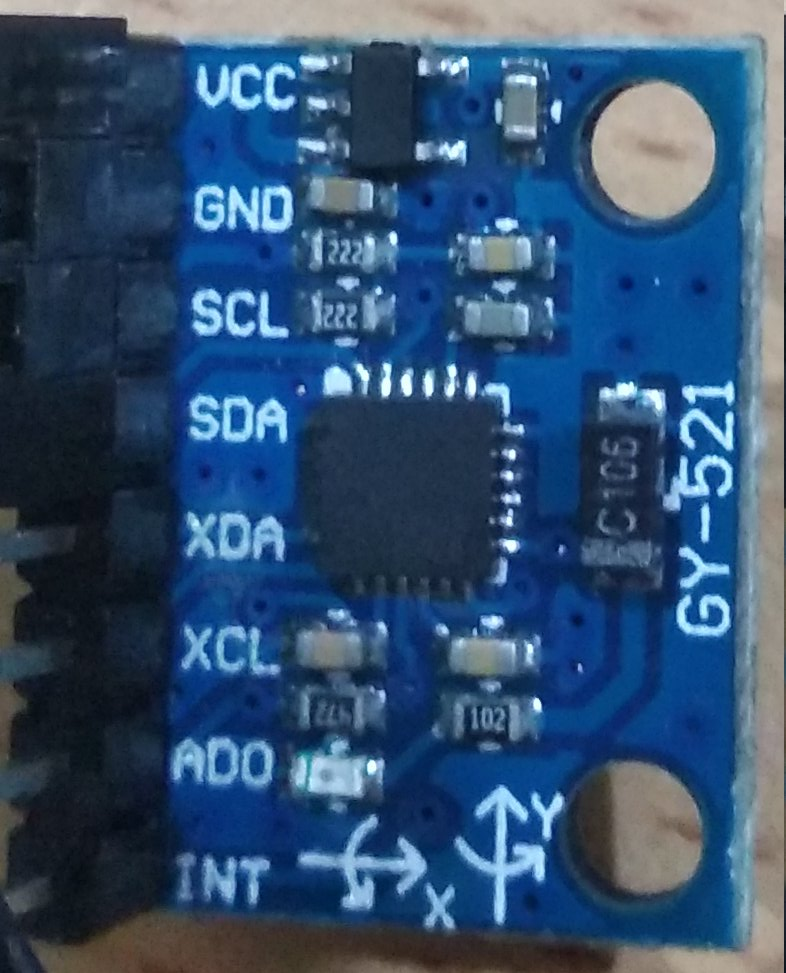
\includegraphics[width=\linewidth]{dokumentasi/MPU6050/mpu6050.jpg}
		\caption{Tampak depan.}
	\end{subfigure}
	\begin{subfigure}[b]{0.35\linewidth}
		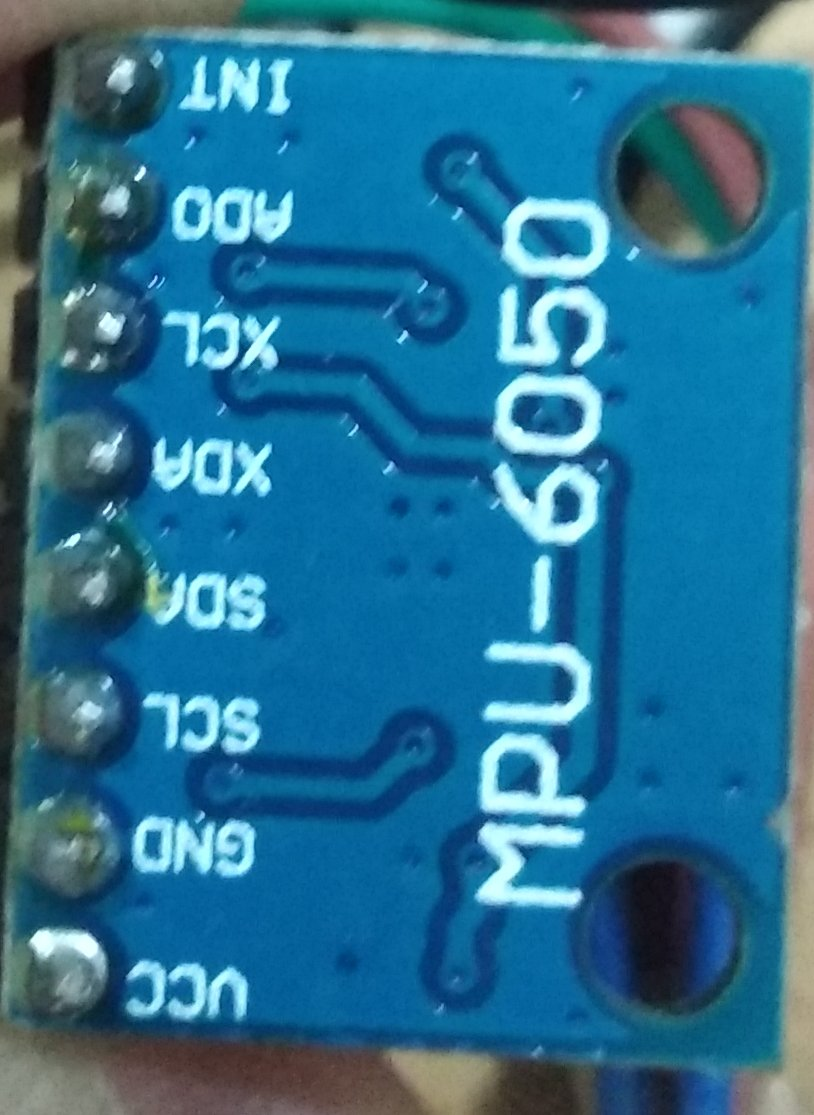
\includegraphics[width=\linewidth]{dokumentasi/MPU6050/mpu60501_1.jpg}
		\caption{Tampak Belakang.}
	\end{subfigure}
	\caption{MPU 6050}
	\label{fig:MPU 6050}
\end{figure}
Cara kerjanya untuk sensor accelorometer ini adalah  adalah menggunakan lempengan.
Lempengan tersebut dialiri aliran listrik.
Ketika terjadi perubahan gerakan pada bagaian-bagaiannya maka bagaian itu terjadi perubahan kapasistif.
Lalu perubahan kapasitif inilah yang menjadi tegangan output.
Untuk gambaran cara kerja untuk sensor acceloromoter bisa dilihat pada gambar 2.2
\begin{figure}[!h]
	\centering
	\captionsetup{justification=centering}
	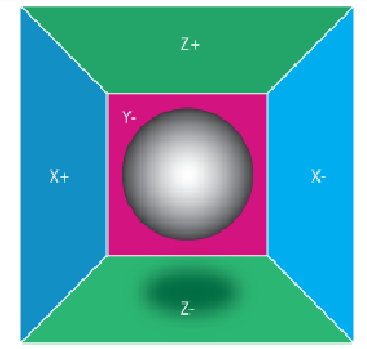
\includegraphics[width=0.7\linewidth]{dokumentasi/MPU6050/contoh.png}
	\caption[Struktur Serat]{\small{Struktur umum serat optik}}
\end{figure}
Pada gambar 2.2 menggambarkan suatu bola pada kotak yang mempunyai sumbu X, Y dan Z. 
Setiap ada gerakan tertentu bolah pasti menyentuh beberapa sumbu tersebut.
Sentuhan bisa pada sumbu X, Y atau Z atau bisa sentuhan tersebut pada sumbu positif atau negatif.
Pada gambar 2.2 karena sudah terintegrasi dengan accelerometer maka modul ini mempunyai 3 sumbu yaitu X, Y dan Z.
Untuk IC yang digunakan adalah MPU 6050.
Chip ini mempunyai banyak fitur salah satunya adalah sudah memiliki digital motion prosesor (DMP) yang mengolah data mentah dari masing-masing sensor dan dapat menimalisasi error yang dihasilkan.

\subsection{Modul Mic Arduino}
Mic adalah suatu perangkat yang mengubah gelombang suara menjadi gelombang elektrik.
Cara kerja mic ini adalah  terdapat membran dan membran inilah yang menghasilkan listrik.
Kecepatan bergeraknya membran inilah yang menghasilkan listrik yang dihasilkan.
Untuk modul dapat dilihat pada \label{fig:MAX9814}.
\begin{figure}[h!]
	\centering
	\begin{subfigure}[b]{0.39\linewidth}
		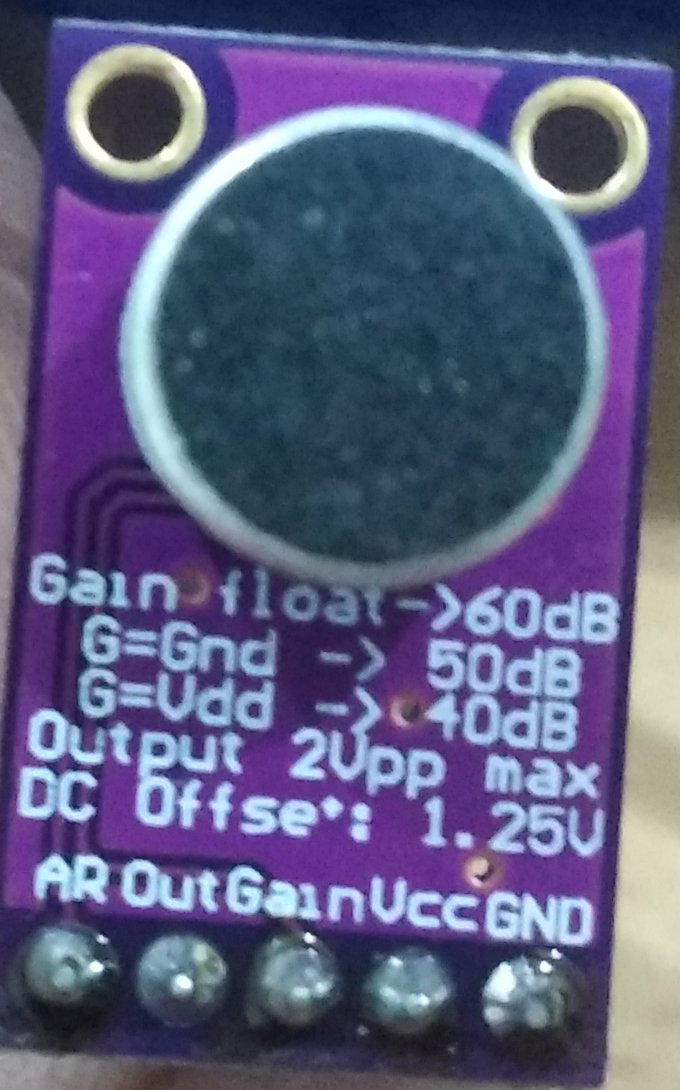
\includegraphics[width=\linewidth]{dokumentasi/MIC/1.jpg}
		\caption{Tampak depan.}
	\end{subfigure}
	\begin{subfigure}[b]{0.4\linewidth}
		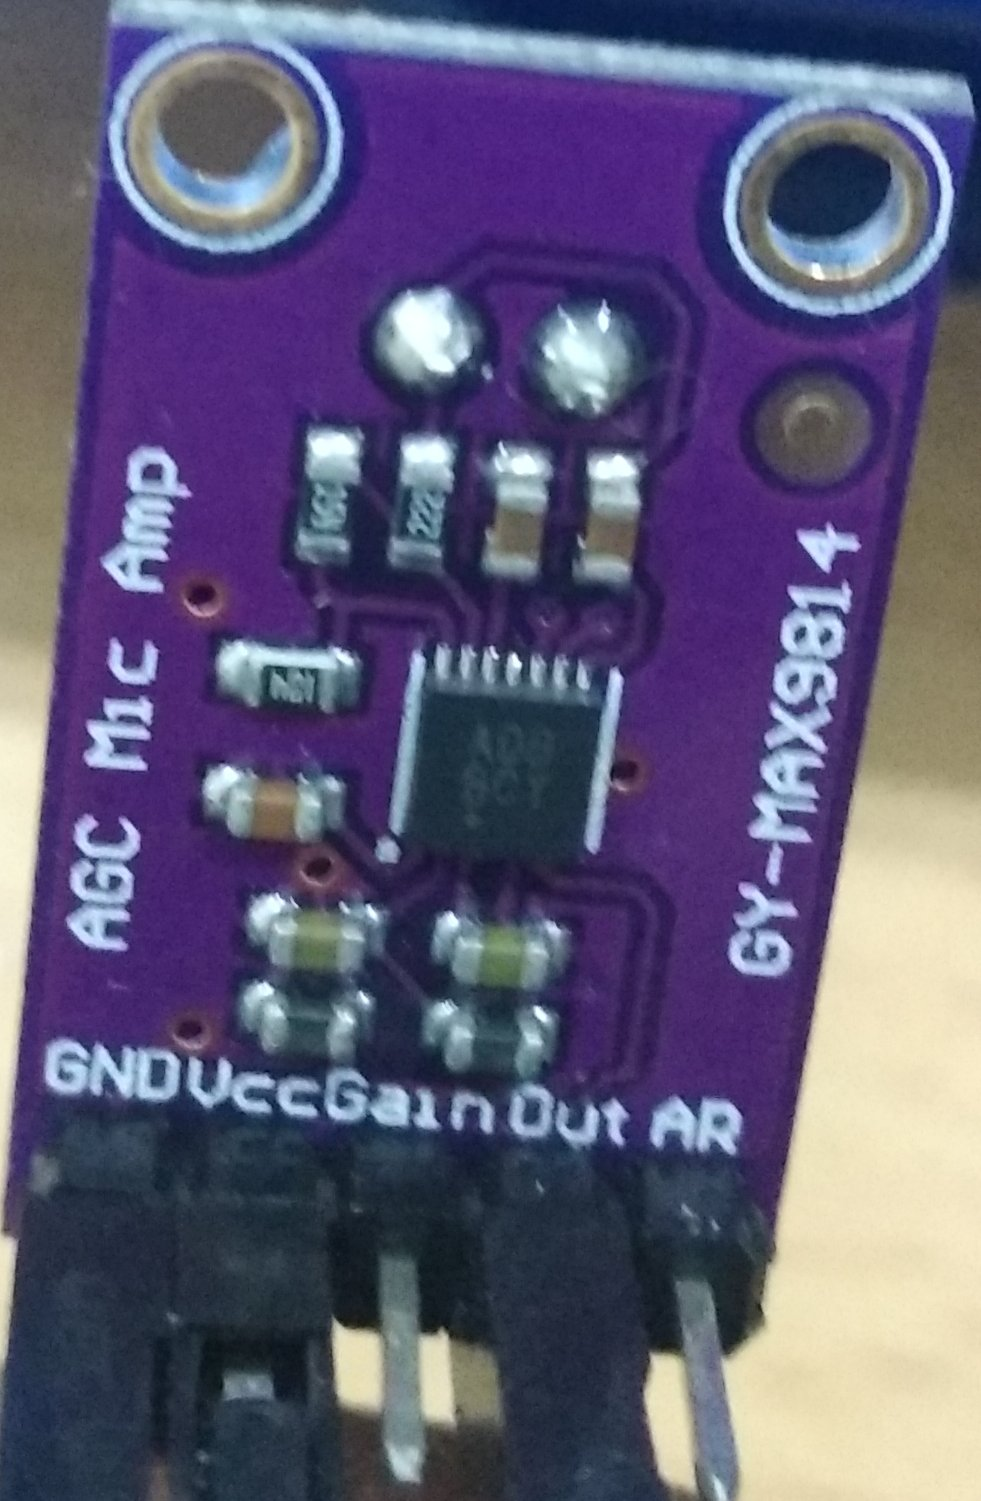
\includegraphics[width=\linewidth]{dokumentasi/MIC/2.jpg}
		\caption{Tampak Belakang.}
	\end{subfigure}
	\caption{MAX9814}
	\label{fig:MAX9814}
\end{figure}
Pada gambar 1.4 adalah modul mic yang menyediakan potensiometer.
Berbagai macam gain dalam modul ini berfungsi sebagai mengubah atau menyesuaikan gain keluaran keluaran.
Keluaran gain ini nantinya akan berpengaruh ke input ADC.
Sinyal yang terhubung dengan modul ini akan merubah dalam bentuk ADC agar bisa dirubah dalam bentuk sinyal digital.

\subsection{Modul Wifi esp 8266}
Modul WI-Fi ESP 8266 adalah sebuah hardrware yang berfungsi untuk menghubungkan suatu mikrokontroller ke internet atau device lain melalui jaringan WI-FI.
Penghubungan ke internet berarti modul ini sebagai akses point.
Namun ketika mengkomunikasikan melalui device lain maka masuk mode AT.
Untuk foto hardware bisa dilahat pada gambar dibawah ini.
\begin{figure}[h!]
	\centering
	\begin{subfigure}[b]{0.39\linewidth}
		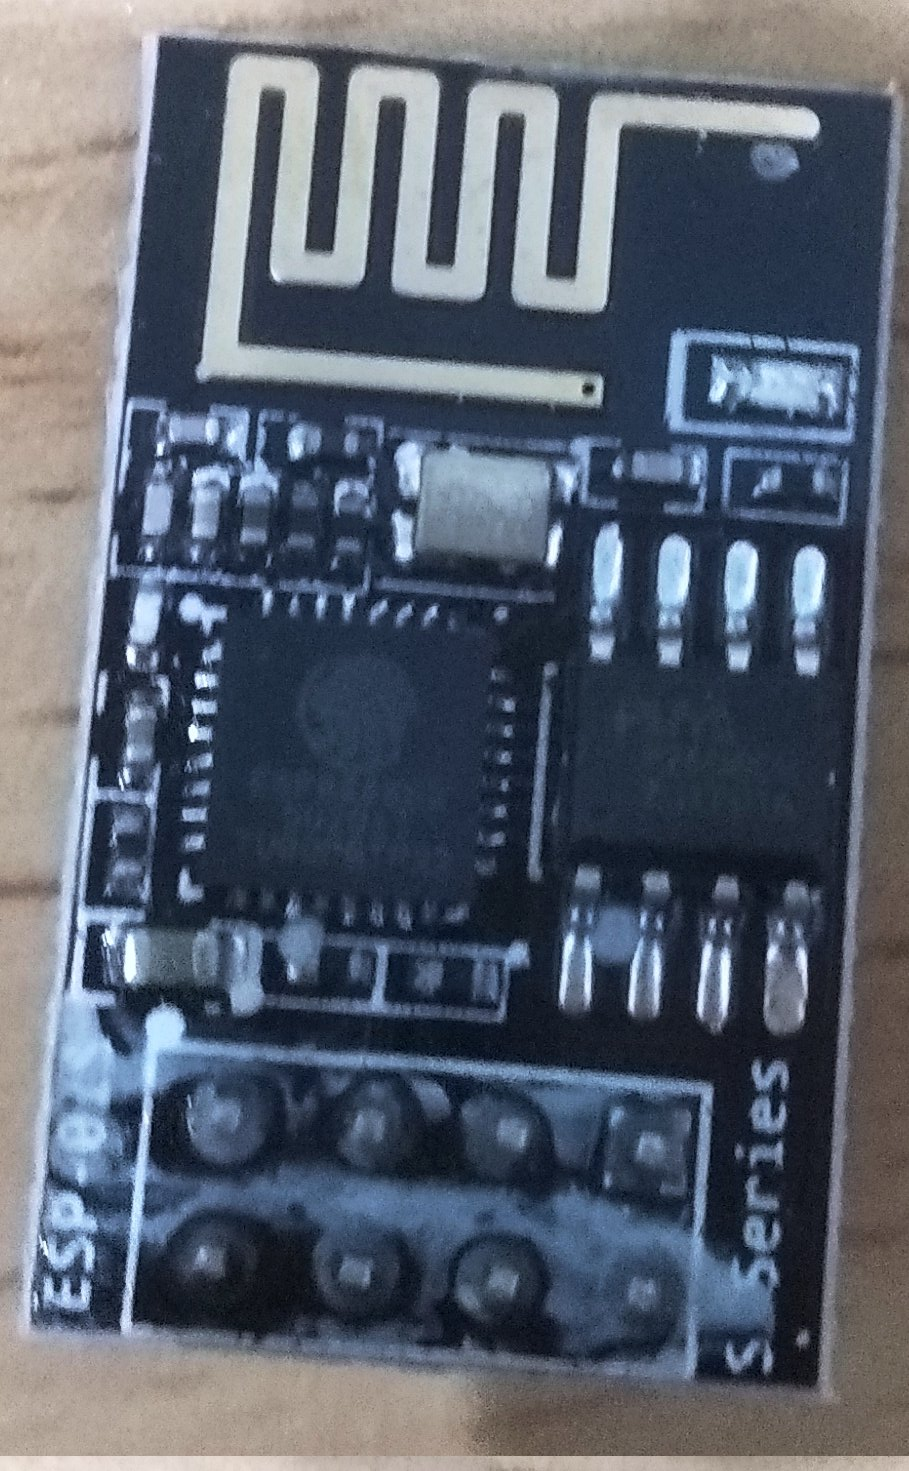
\includegraphics[width=\linewidth]{dokumentasi/ESP8266/wifi2.jpg}
		\caption{Tampak depan.}
	\end{subfigure}
	\begin{subfigure}[b]{0.4\linewidth}
		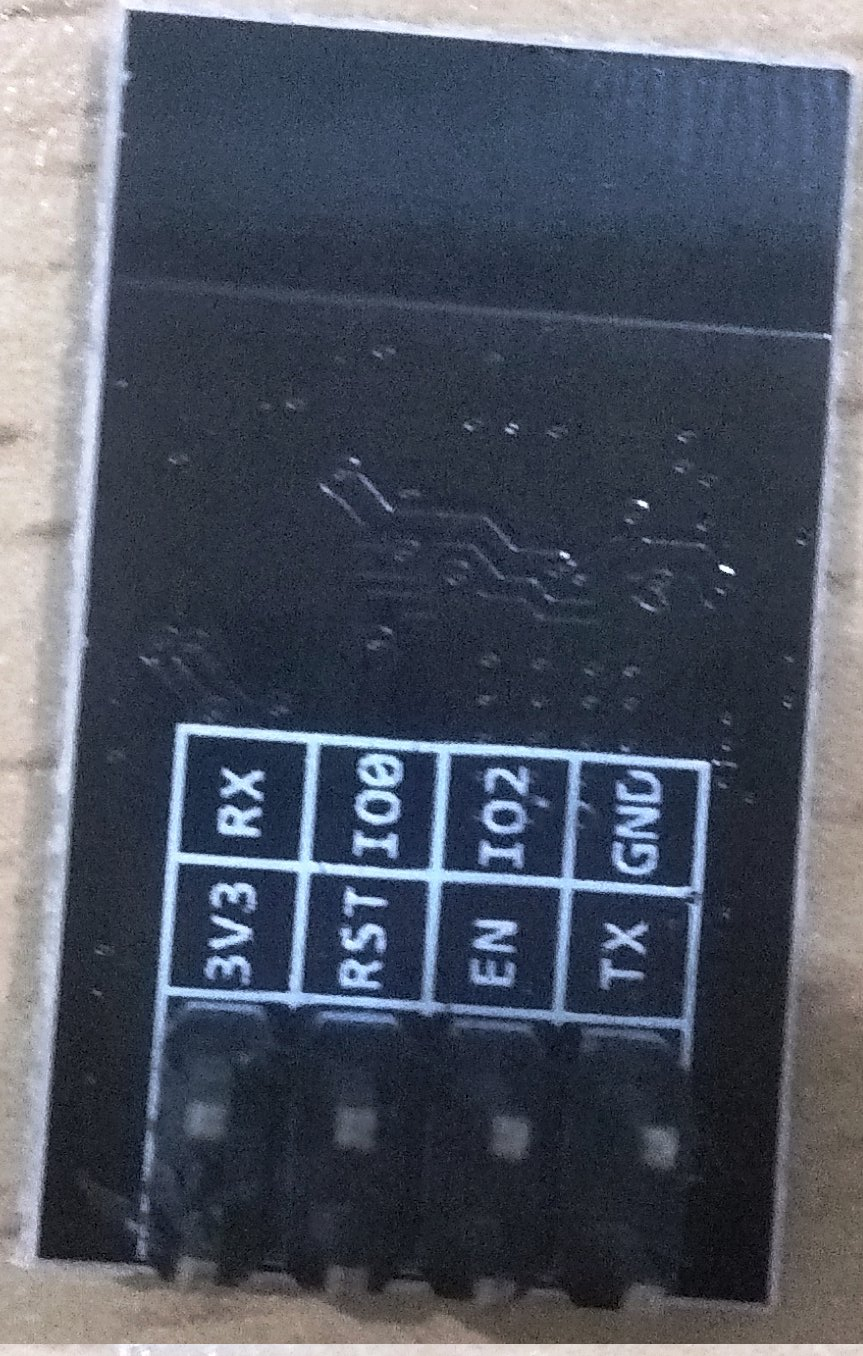
\includegraphics[width=\linewidth]{dokumentasi/ESP8266/wifi1.jpg}
		\caption{Tampak Belakang.}
	\end{subfigure}
	\caption{ESP8266}
	\label{fig:ESP8266}
\end{figure}
Penggunaan komunikasi dengan ESP 8266 adalah dengan memberikan \textit{jumper} pada bagaian bagaian berikut: 
\begin{table}[h!]
	 \caption{Komukasi ESP 8266.}
	\label{tab:Komukasi ESP 8266}
	\begin{tabular}{|l|l|lll}
		\cline{1-2}
		ESP8266 & STM 32 &  &  &  \\ \cline{1-2}
		Ground  & Ground &  &  &  \\ \cline{1-2}
		Vin     & 3,3 V  &  &  &  \\ \cline{1-2}
		Enable  & 3,3 V  &  &  &  \\ \cline{1-2}
		TX  	& RX  	&  &  &  \\ \cline{1-2}
		RX  	& TX V  &  &  &  \\ \cline{1-2}
	\end{tabular}
\end{table}
Pada Tabel bisa dilihat untuk sinyal pemberi untuk ESP8266 dihubungkan dengan sinyal penerima pada STM 32.
Begitu pula dengan sinya penerima pada ESP 8266 dihubungkan dengan STM 32. hal ini dilakukan komunikasi bisa berlangsung.
Karena dalam mengirim data client harus meminta permintaan data dahulu pada server.
Setelah permintaan data sudah diterima maka pengiriman data baru bisa dilakukan.
\subsection{Modul Charger Baterai}
Pada modul berfungsi sebagai kontrol tegangan dan arus sebelum masuk ke baterai.
Tegangan pada micro USB adalah 5 VDC sedangkan pada tegangan  baterai adalah 3.7.
VDC namun dalam percobaan tegangan ketika charging adalah 4,2 VDC.
\begin{figure}[!h]
	\centering
	\captionsetup{justification=centering}
	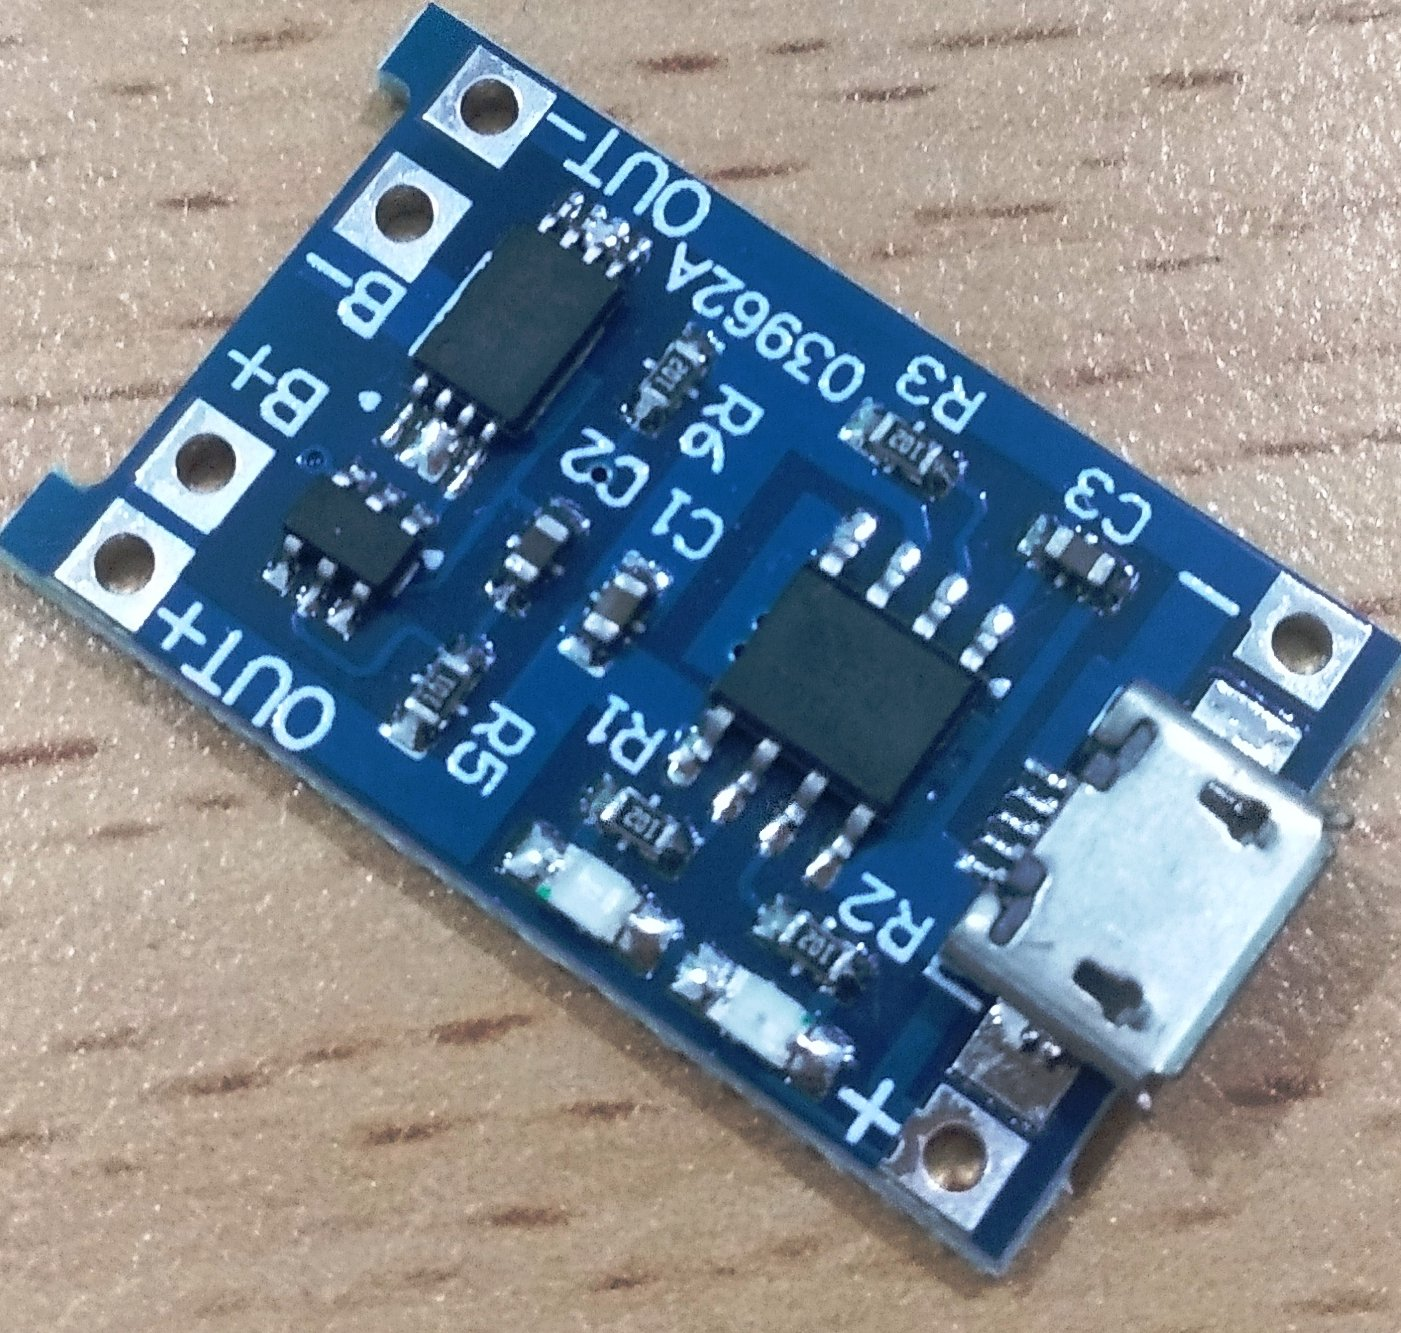
\includegraphics[width=0.7\linewidth]{dokumentasi/modulcharging.jpg}
	\caption[modulcharging]{\small{modulcharging}}
\end{figure}
Pada gambar menunjukkan tentang modul chager pada baterai lithium 3.7V.
Dalam modul charger tersebut ada 3 IC utama yang tertanam dalam modul tersebut.\cite{For2011}
3 IC tersebut adalah  IC dengan jenis LTC4056-4.2 lalu IC dengan jenis DWG01 dan IC dengan jenis S-8205A/B.
Untuk penjelasannya IC  LTC4056-4.2 berfungsi mengubah tegangan input dengan masukan 4,5-6,5V menjadi tegangan charging 4,2 V dengan arus ke baterai sesuai datasheet 700 mA\cite{LTC2018}.
IC kedua alah IC DWG01-G yang berfungsi mempertahankan tegangan di 4,2 V\cite{For2011}.
Pada IC S-8205A/B adalah IC yang memberikan pengamanan listrik pada baterai\cite{Ic2016}

\subsection{Modul Step Up Tegangan 5V}
Modul step up ini adalah merubah tegangan dari baterai menjadi tegangan operasional pada microcontreller.
Perubahan tegangan ini diperlukan karena tegangan operasional baterai adalah 3.7 VDC dan untuk tegangan operasional pada mikrokontroller adalah 5VDC.
Pada modul step up ini tertanam IC 
\begin{figure}[!h]
	\centering
	\captionsetup{justification=centering}
	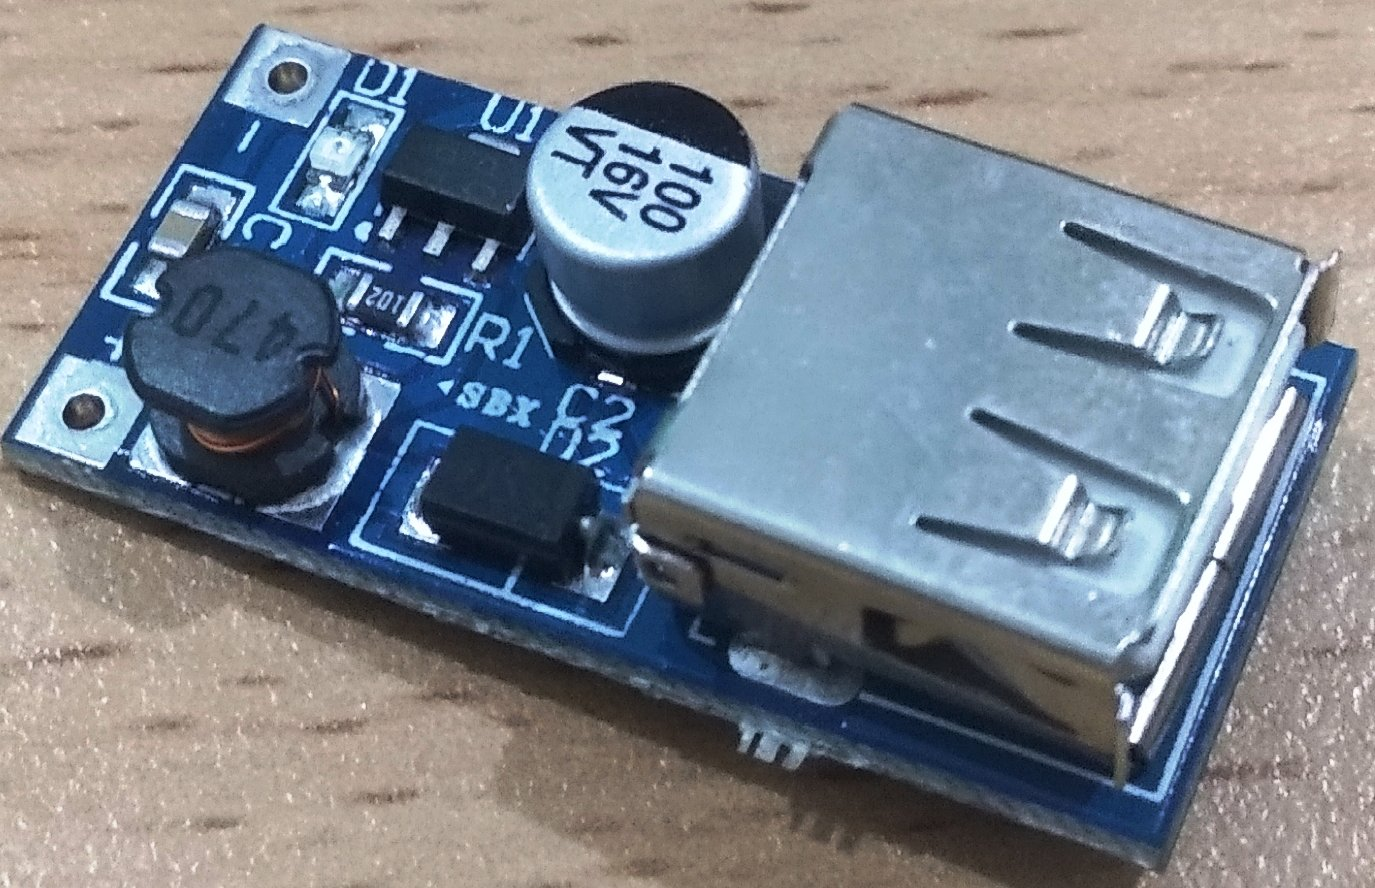
\includegraphics[width=0.7\linewidth]{dokumentasi/modul5v.jpg}
	\caption[modulcharging]{\small{modul 5V}}
\end{figure}
\subsection{Baterai Lithium 3,7 V}
Baterai adalah tempat penyimpanan energi listrik melalui reaksi kimia. 

\subsection{STM32}

\subsection{ChibiOS/RT}

\subsection{Fuzzy}
alkan konsep kebenaran sebagaian.
Konsep ini menyatakan segala hal bisa di istilahkan dalam binary yaitu 1 dan 0.
Dalam hal ini logika fuzzy menggantikan teoti boolean dalam tingkat kebenaran.
Dalam logika fuzzy nilai keanggotaan dapat dikelompokkan seperti rendah, sedang dan sangat tinggi.
Untuk lebih jelasnya proses fuzzyfikasi bisa dilihat pada gambar 1.4

Pada gambar menerangkan tentang diagram alir proses dari fuzzy. Penjelasannya adalah sebagai berikut;
\begin{enumerate}[label=\alph*.]
	\item Input. Bilangan crisp yang berisi nilai dari suatu nilai input. Nilai input yang berisi tentang \textit{objectif function} yang akan diproses
	\item Fuzzyfication. Fungsi ini berguna mengkonversi atau mengubah bilangan crisp menjadi bilangan fuzzy.
	\item Rule Base \& Inference System. adalah dimana suatu proses pengaturan fuzzy antara input 1 dan input 2 dengan output. Pengaturan tersebut lebih ke "jika" dan "maka"
	\item Defuzzyfication adalah perubahan nilai \textit{output} berupa keanggotaan keluaran
	\item Output adalah hasil mitigasi yang harus dilakukan.
\end{enumerate}
Pada Gambar 1.5 terlihat mekanisme dari proses dari input yang dibutuhkan untuk fuzzy logic dari data awal sampai dari hasil fuzzy logic.
Untuk yang pertama data-data yang dibutuhkan adalah data batasan untuk setiap kelompok cluster sehingga nantinya dikelompokan menurut kategorinya.
Pada sebuah himpunan fuzzy  direpresentasikan pada fungsi keanggotaan gaussian, generalized bell ataupun segitiga.
Contoh penjelasannnya adalah sebgai berikut:
\begin{enumerate}[label=\alph*.]
	\item Fungsi keanggotaan segitiga, Fungsi  keanggotaan  segitiga dibentuk oleh 3 parameter  {a, b, c} yang dapat dideskripsikan oleh Persamaan (2.4)
	
	\begin{equation}
		\mu[x] = 0;x \leq a
	\end{equation}
	
	\begin{equation}
		\mu[x] = 0;x \geq a
	\end{equation}
	
	\begin{equation}
		\mu[x] = \frac{(x-a)}{(b-a)};a < x \leq b
	\end{equation}
	
	\begin{equation}
		\mu[x] = \frac{(c-x)}{(c-b)};b < x \leq c
	\end{equation}
	
	\begin{equation}
		\mu[x] = \max(\min(\frac{(x-a)}{(b-a)} , \frac{(c-x)}{c-b}), 0)
	\end{equation}
	
	\item Fungsi Keanggotaan Trapesium, fungsi keanggotaan trapesium dibentuk oleh 4 parameter {a, b, c, d} yang dapat dideskripsikan oleh Persamaan (2.5)
	\item Fungsi keanggtaan gaussian. Fungsi  keanggotaan  Gaussian  dibentuk  oleh  2  parameter .	c merpresentasikan pusat fungsi keanggotaan dan \ merepresetasikan lebar ruang fungsi  keanggotaan.
	Fungsi  keanggotaan  Gaussian  dapat  dideskripsikan  oleh Persamaan (2.6)
	\item d. Fungsi keanggotaan generalized bell. Fungsi keanggotaan generalized bell dibentuk oleh 3 parameter {a, b, c} dimana nilai b bernilai positif dan nilai b negatif mengakibatkan kurva terbuka ke atas.  Fungsi  keanggotaan  generalized  bell  dapat  dideskripsikan  oleh  Persamaan (2.7)
	\item Output adalah hasil mitigasi yang harus dilakukan.
\end{enumerate}

\subsection{Particle Swarm Optimization}
PSO yang mempunyai kepanjangan Particle Swarm Optimization adalah sistem yang menggunakan salah satu sistem optimasi yang terinspirasi oleh kumpulan burung dan ikan [16].
Dalam cara kerjanya partikel atau keanggotaan ini mencari kecepatan dan tempat terdekat untuk makannya.
Dalam hal ini makanannya berarti tujuan dari partikel-partikel tersebut. 

Pada gambar 1.5 menjelaskan tentang fungsi minimal pada pergerakan partikel.
Pada dasarnya sistem optimasi ini dituntut untuk mencari kecepatan terbaik dan jarak terpendek pada tujuan yag telah ditentukan.
Suatu individu atau partikel ditentukan  dan posisi diartikan  sebagai vector.
Jadi pada PSO digunakan untuk mencari nilai titik optimum pada data yang ada.
Untuk diagram alir bisa dilihat pada gambar 1.8 dan 1.9

Pada gambar 1.8  dalam optimasi variable setiap data pasti berubah sehingga partikel akan mengingat posisi terbaik dan kecepatan terbaik berdasarkan informasi yang diterima.
Biaanya dalam kawanan burung akan mengikuti batasan seperti seekor burung tidak akan terlalu dekat atau terlalu jauh dengan yang lain.
Setiap burung akan mengarahkan mengikuti arah kawanan burung yang lain

PSO merupakan metode optimasi artificial intelligence yang  mengadopsi perilaku sosial kawanan burung atau ikan.
Perilaku sosial dari organisme tersebut baik individu maupun kawanan (swarm) dijadikan sebagai dasar dalam merancang algoritma PSO.
Setiap solusi dapat dianggap sebagai partikel atau seekor burung.
Burung akan mencari makanannya melalui usahanya sendiri dan kerja sama sosial dengan kawanannya.
Algoritma PSO  pertama  kali diperkenalkan  oleh  R.  Eberhard  dan  J.  Kennedy  pada  tahun 1995.
Gambar 2.11 merupakan algoritma standar dari Particle Swarm Optimization.
Banyak ilmuan yang telah memodifikasi PSO baik dari kecepatan partikel maupun dari bobot inersia.
Salah satunya adalah Linear Decreasing Particle Swarm Optimization (LDWPSO).
Algoritma LDWPSO memodifikasi nilai dari bobot inersia PSO original.
Dengan mengganti persamaan nilai bobot inersia menjadi persamaan berikut :
Algoritma ini pernah dipakai oleh Alrijadjis Djoewahir untuk meningkatkan Stabilitas dan akurasi Ultrasonic Motor (2012) dan hasilnya meningkat secara signifikan.
%=============================================================================

%\newpage
%\thispagestyle{plain}
%\mbox{} 

%=============================================================================
% BAB III 

\newpage

\setcounter{figure}{0}

\section{Metodologi Penelitian}

\begin{center}
	{\large \textbf{BAB III}} \\
	{\large \textbf{Metodologi Penelitian}}
\end{center}

Tahapan-tahapan yang akan dilaksanakan pada tugas akhir ini adalah sebagai berikut :
\subsection{Studi Literatur}

Studi literatur digunakan untuk meningkatkan pemahaman peneliti mengenai topik yang dipilih. Studi literatur dilakukan dengan mempelajari hal – hal yang mendukung selama penelitian seperti Fuzzy dan sistem optimasi. Hal ini digunakan untuk mendetailkan dan gambaran tugas akhir kedepannya  sehingga dalam perjalanan

\subsection{Menentukan Kegiatan Pengambilan Data}

\subsection{Perancangan Alat}
Pada perancangan alat untuk deteksi jatuh dibutuhkan sensor accelerometer dan gyroscope,
STM 32, modul Wifi dan Android sepert pada gambar dibawah ini.


Pada Gambar 1.7 penggunaan sensor digunakan sebagai posisi pada sumbu X, Y dan Z.
posisi ini digunakan sebagai apakah objek dalam posisi berdiri, duduk, tertidur ataupun posisi lainnya seperti jongkok.
Lalu ditambahkan sensor suara untuk mempertambah ke akurasian untuk sensor jatuh ini.
Lalu nilai yang keluar dari sensor diteruskan dan diproses oleh accelorometer.
STM 32 tersebut akan memproses secara fuzzy PSO.
Setelah pemrosesan dalam fuzzy PSO maka apakah posisi objek tersebut terjadi jatuh secara valid atau tidak. Jika posisi objek jatuh dan dinyatakan valid maka arduino mengirimkan sinyal ke ke modul Wi-Fi dan diteruskan ke router yang tersambung internet. 
Dari komunikasi Wi-fi tersebut mengirimkan sinyal dan pemberitahuan ke ponsel android yang terhubung,

\subsection{Realisasi Alat}

\subsection{Pengambilan data}

\subsection{Perancangan fuzzy}

\subsection{Perancangan PSO}

\subsection{Pengujian Alat}

DalamPengambilan data ini sangat penting untuk melakukan ujihardware dan software agar kinerjanya sesuai dengan harapan.
Pengujiannnya untuk sistem berfungsi dari angka 0 sampai 100%  mempunyai 2 kategori.
Penilaian pertama yaitu sensitifitas.
Sensitifitas adalah seberapa  besar untuk mengklasifisasikan pengambilan keputusan tersebut dengan benar.
Sensitifitas dapat dihitung dengan rumus  dengan persamaan 1.1

Pada persamaan 1.1 yang dimaksud dengan positif benar adalah keputusan atau notifikasi yang benar akan keadaan yang ada.
Contohnya ketika sistem memberi notifikasi terjadinya objek yang jatuh dan di lapangan terjadi objek yang jatuh maka hal termasuk positif benar.
Namun ketika terjadi notifikasi objek yang jatuh tetapi pada dilapangan ternyata objek tidak terjatuh (objek melakukan kegiatan sehari-hari) maka hal ini disebut negatif palsu.
Spesitifitas adalah adalah tidak ada notifikasinya jatuh dan memang benar dilapangan objek tersebut memang tidak jatuh. Untuk rumus untuk spesitifitas dirumuskan pada persamaan 1.2

Pada persamaan 1.2 maksud dari negatif benar adalah kejadian yang tidak jatuh dan benar sistem mendeteksi kejadian tersebut termasuk kegiatan sehari-hari dan bukan kegiatan terjatuh.
Untuk positif palsu adalah saat objek benar-benar terjatuh namun dalam sistem tidak ada notifikasi 
%=============================================================================
% Daftar Pustaka
\newpage

\section{Daftar Pustaka}

\begin{center}
	\textbf{Daftar Pustaka}
\end{center}

	\bibliographystyle{IEEEtran}
	\bibliography{/home/zain/Documents/didinTA/latex/library.bib}

\end{document}